\documentclass[12pt,openany,final]{book}
\usepackage[letterpaper,margin=1in,footskip=0.25in]{geometry}
\fontfamily{cmr}
\usepackage[final]{changes}
\usepackage{lipsum}
\usepackage[nottoc]{tocbibind}
\usepackage[T1]{fontenc}
\usepackage[utf8]{inputenc}
\usepackage{flafter}
\usepackage{floatrow}
%\usepackage{floatflt}
\usepackage{placeins}
\usepackage{siunitx}
\usepackage{graphicx}
\graphicspath{{figures/}}% Include figure files
\usepackage{dcolumn}% Align table columns on decimal point
\usepackage{appendix}
\usepackage{amsmath}
\usepackage{cases}
\usepackage{calc}
\usepackage{amssymb}
\usepackage{color}
\usepackage{enumitem}
\usepackage{soul}
\usepackage{indentfirst}
\usepackage{hyphenat}
\usepackage{xspace}
\usepackage{subcaption}
\usepackage{booktabs}
\usepackage{multirow}
\usepackage{tabularx}
\usepackage{xcolor}
\usepackage{lineno}
\usepackage{setspace}
\usepackage{titlesec}
\usepackage{hyperref}
\usepackage[superscript]{cite}
\usepackage{lineno}
\titleformat
{\chapter} % command
[display] % shape
{\sc\LARGE} % format
{Chapter \thechapter} % label
{0.2ex} % sep
{
} % before-code
\titlespacing*{\chapter}{0pt}{1in}{0pt}
\titlespacing*{\section}{0pt}{0pt}{0pt}
\hbadness=99999
%\epstopdfDeclareGraphicsRule{.tga}{png}{.png}{
%    convert #1 \OutputFile
%}
\hypersetup{
    colorlinks,
    citecolor=black,
    filecolor=black,
    linkcolor=black,
    urlcolor=black
}
%\newcommand{\cmpersec}{$\frac{\text{cm}}{\text{s}}$~}
\newcommand{\cmpersec}{cm/s~}
\newcommand{\etal}{\textit{et al.}}
\newcommand{\na}{Na\textsuperscript{+}~}
\newcommand{\cl}{Cl\textsuperscript{-}~}
\newcommand{\PM}{$\pm$~}
\newcommand{\invnm}{$\text{\si{\nm}}^{-1}$~}
\newcommand{\nmeter}{\si{\nm}~}
\renewcommand{\arraystretch}{1.8}
%\newcommand{\hl}{\added}
%\newcommand{\sout}{\deleted}
\newcommand{\TODO}{\hl{TODO}~}
\newcommand{\about}{$\sim$}
\newcommand{\aangstroms}{{\aa}ngstr{\"o}ms}
\newcommand{\aangstrom}{{\aa}ngstr{\"o}m}
\newenvironment{hle}{\color{red}}

\newcommand{\beginsupplemental}{%
    \setcounter{table}{0}
    \renewcommand{\thetable}{S\arabic{table}}%
    \setcounter{figure}{0}
    \renewcommand{\thefigure}{S\arabic{figure}}%
}

\author{Matthew Saunders}
\title{Modeling Interactions of Ions with Ether- and Ester-linked Phospholipids}
\begin{document}
\pagestyle{plain}
%\maketitle
\begin{titlepage}
\begin{centering}
~\\[1in]
Modeling of Interaction of Ions \\[2\baselineskip] with Ether- and Ester-linked phospholipids
~\\[3\baselineskip]
by
~\\[3\baselineskip]
Matthew W. Saunders
~\\[4\baselineskip]
A thesis submitted in partial fufillment\\
of the requirements of the degree of\\
Master of Science in Biology \\ with a concentration in Cell \& Molecular Biology\\
Department of Cell Biology, Microbiology and Molecular Biology\\
College of Arts and Sciences\\
University of South Florida\\
~\\[2\baselineskip]
Major Professor: Sameer Varma, Ph.D.\\
Sagar Pandit, Ph.D.\\
H. Lee Woodcock, Ph.D.\\
Jianjun Pan, Ph.D.\\
~\\[2\baselineskip]
%Date of Approval:\\
%XXX\\
~\\[3\baselineskip]
\end{centering}
\end{titlepage}
\doublespacing
\tableofcontents
\pagenumbering{roman}
\listoftables
\listoffigures
\bibliographystyle{elsarticle-num}
%\linenumbers
\doublespacing
\chapter*{Abstract}
\addcontentsline{toc}{chapter}{Abstract}

Polar lipids, or phospholipids, are present in all parts of cells
and are used in many signalling and structural roles.
As structural molecules they act as the main component of cellular plasma membranes --- bilayers
of polar lipids that separate cells from their environments. Bilayer properties are heavily
influenced by the structure of their component polar lipids, and different lipids
are found in different organisms. 
A distinguishing feature of Archaeal plasma membranes is that their phospholipids contain ether-links, as opposed to bacterial and eukaryotic plasma
membranes where phospholipids primarily contain ester-links. In our work we examine the effects of
salt on bilayer structure in the case of an ether-linked lipid bilayer. We use molecular dynamics simulations and compare equilibrium properties of two model lipid
bilayers in NaCl salt solution --- POPC and its ether-linked analog that we refer to as HOPC. We make the following key observations.
The headgroup region of HOPC ``adsorbs'' fewer ions compared to the headgroup region of POPC. Consistent with this,
we note that the Debye screening length in the HOPC system is \about 10\% shorter than that
in the POPC system. Herein, we introduce a protocol to identify the lipid-water interfacial boundary that
reproduces the bulk salt distribution consistent with
Gouy-Chapman theory. We also note that the HOPC bilayer has excess solvent
in the headgroup region when compared to POPC,
coinciding with a trough in the electrostatic potential. Waters in
this region have longer autocorrelation times and smaller lateral diffusion rates compared to the corresponding region
in the POPC bilayer, suggesting that the waters in HOPC are more strongly
coordinated to the lipid headgroups. Furthermore, we note that it is this
region of tightly coordinated waters in the HOPC system that has a lower density of Na$^+$ ions.
Based on these observations we conclude that an ether-linked lipid bilayer has a lower binding
affinity for Na$^+$ compared to an ester-linked lipid bilayer.

\chapter{Introduction}
\linenumbers
\pagenumbering{arabic}

\section{Ether- and Ester-linked Phospholipids}
Phospholipids are a diverse species of biological molecules used in many roles in life~\cite{van:2008:lipidvariety}. These molecules
are amphipathic, with a headgroup that is hydrophillic attached to hydrophobic acyl chains by a
glycerol backbone~\cite{pandit:2008:simulationtextbook,israelachvili:2011:intermol}. 
These molecules, when above a critical concentration in aqueous solution, self assemble into
various aggregate structures in order 
to reduce the exposure of the hydrophobic chains
to polar solvent --- these structures include
micelles, vesicles, and bilayers along with others~\cite{israelachvili:2011:intermol}. 
Phospholipids tend to form bilayers, 
where the hydrophillic headgroups face the solvent and the 
hydrophobic acyl chains face into the center 
of the structure~\cite{israelachvili:2011:intermol,ashrafuzzaman:2012:membrane}. 
An image of a bilayer of a commonly studied
model lipid can be seen
in figure~\ref{fig:boximage}.
\begin{figure}[p]
    \caption[Image of a model bilayer of phospholipids from a simulation.]{ Image of a model bilayer of phospholipids from a simulation. The lipids can be seen
in the center of the image, with the hydrophobic chains colored in
light purple. The polar headgroup can be seen highlighted by the phosphate group in orange and the choline nitrogen in blue
facing the solvent. Solvent molecules have been removed for clairity. Figure generated
using VMD~\cite{vmd}}
\label{fig:boximage}
\includegraphics[width=\textwidth]{images/popc_image}
\end{figure}
In living cells, lipid bilayers act as the delimiter between the cell and the environment, acting as one of the major constituients of the cellular 
plasma membrane~\cite{reece:2014:biobook}. The plasma membrane consists of a mixture of many lipid species, as
well as proteins and lipid-like molecules, and the mixture is tuned by the cell to adapt the 
structure and flexibility of the plasma membrane to different environments~\cite{pandit:2008:simulationtextbook,van:2008:lipidvariety,zhang:2008:memhomeo}. 
Furthermore, the cellular membrane is the interface for exchange
of nutrients with the environment, and also the interface for the transmission of signals to and from the outside of the cell. This
exchange is done through passive diffusion, proteins and other molecules embedded into the membrane, and through the formation
of vesicles and buds out of the lipid bilayer~\cite{reece:2014:biobook}. The behavior and function of the plasma membrane
is heavily dependent on the structure of the bilayer, which again can be influenced directly by the mixture of phospholipids constituting the
membrane~\cite{van:2008:lipidvariety,zhang:2008:memhomeo}.

Phospholipids can be modified in a variety of ways to change their chemical construction,
and the structure of the individual molecules manifest significant changes
in the stucture of aggregates, like lipid bilayers or cell membranes.
Polar headgroups can be charged or zwitterionic~\cite{israelachvili:2011:intermol}. The fatty acid chains can be saturated or unsaturated, 
and can have many lengths depending 
on the needs of the cell --- differing the acyl chains influences the 
phase behavior of the bilayer, which can help cells to adapt to changes in
temperature~\cite{ashrafuzzaman:2012:membrane,zhang:2008:memhomeo}.

Phospholipids can also use several types of chemical links between the glycerol
backbone and the fatty acid chains~\cite{sehgal:1962, koga:2014}.
Phospholipids containing ether-links represent one of the many major evolutionary divides -- 
while they make up much of the phospholipids of archaeal membranes,
 they are present in only small fractions in eukarya and bacteria~\cite{sehgal:1962, koga:2014, kates:1993:archealipids}. 
These phospholipids differ from the more common ester-linked phospholipids of bacterial and 
eukaryotic membranes in that they lack fatty acid carbonyl groups (see figure \ref{fig:struc}). 

\begin{figure}[p]
\caption[Chemical structures of representative phospholipids highlighting the difference
between ether- and ester-links.]{ 
Chemical structures of representative phospholipids highlighting the difference 
between ether- and ester-links. POPC (1-palmitoyl-2-oleoyl-sn-glycero-3-phosphatidylcholine) is a 
diester lipid and HOPC (1-hexadecyl-2-(9-octadecenyl)-sn-glycero-3-phosphatidylcholine) is its diether analog that lacks fatty acid carbonyl groups.
}
\label{fig:struc}
\includegraphics[height=0.66\textheight]{images/Structure_annotated}
\end{figure}

The chemical difference between ester- and ether-linked lipids has been shown to influence 
bilayer properties including both structure and permeability~\cite{guler:2009,jansen:1995, gawrisch:1992,haas:1990,fogarty:2015,kruczek:2017:ether}. 
Experiments show that model bilayers composed exclusively of ether-linked lipids have smaller dipole potentials compared to 
bilayers composed of their ester-linked analogs~\cite{gawrisch:1992}; a result also predicted by a molecular dynamics (MD) 
study done by our group~\cite{kruczek:2017:ether}. The interfacial water in ether-linked lipid bilayers is also more structured compared to that 
in ester-linked lipid bilayers, as observed in NMR experiments in the form a larger quadrupolar splitting constants~\cite{gawrisch:1992}, and as 
also reproduced in our simulations~\cite{kruczek:2017:ether}. Two independent experimental studies also show 
that ether-linked lipid bilayers are less permeable to water compared to bilayers composed of their ester-linked 
analogs~\cite{jansen:1995, guler:2009}. 

Nevertheless, all studies aimed at examining differences between ester- and ether-linked lipid bilayers have been carried out in pure water, except for the one recent study by 
Leonard \etal~\cite{leonard:2018}. As such, several studies show that salt significantly 
affects the properties of ester-linked lipid bilayers~\cite{kruczek:2019,kruczek:2017, duro:2016,pabst:2007,sachs:2004,petrache:2006:swelling}. 
For example, in our previous works on the interactions of monovalent and divalent ions on zwitterionic ester-linked lipid bilayers~\cite{kruczek:2019,kruczek:2017}
we found that monovalent cations insert into headgroup region. 
We reported reduction in area per lipid, increase in  bilayer thickness, increased range of ordered solvent at the bilayer surface, and an increase in
the electrostatic dipole potential of the bilayer.
Despite the work done on these lipids in the past, the question of how ions interact with bilayers of ether-linked
phospholipids compared to ester-linked remains a topic of interest.

%\section{Models of Ion-Membrane Interactions - Poission-Boltzmann Theory}
%Ion-bilayer interactions are often modelled in the context of Poisson-Boltzmann theory, which
%expresses ions as a uncorrelated gas, moving through a dielectric continuum~\cite{israelachvili:2011:intermol}.


\section{Using Molecular Dynamics to Study Biological Membranes}
In order to explore the question of how ions interact with bilayers of ether- and ester-linked lipids, we utilize 
Molecular Dynamics (MD) simulations.

Computational methods like molecular often have to strike a balance between accuracy and computational feasibility --- approximations
to the interactions in a system can significantly reduce computational cost, and if carefully done can still result in
accurate reproduction of experimental results~\cite{pandit:2008:simulationtextbook}.

Molecular dynamics approximates systems by treating particles classically. Particles are expressed as points in space, 
with masses centered at the nucleus~\cite{pandit:2008:simulationtextbook}.
Functional forms and terms to calculate the potential energy of systems are defined in a force-field.
Bonds and bond angles in molecules are modeled as harmonic potentials, and torisional parameters within molecules are modeled
using periodic functions. Non-bonded interactions
are modeled using simple pairwise-additive potentials and in general do not treat many-body interactions~\cite{tieleman:1997:memsim,pandit:2008:simulationtextbook}. 
Van der Waals (VdW) dispersion and hard-shell repulsion are usually treated using a Lennard-Jones 6-12 potential,
and short-range electrostatics are represented by a coulomb potential~\cite{tieleman:1997:memsim,pandit:2008:simulationtextbook}.
The potential terms are added together over the whole system of particles
to get the overall potential function of the system, which is then used to evolve the system over time by integrating
Newton's laws of motion~\cite{frenkel:2001:molsimbook}. An example of the total potential can be seen in equation~\ref{eq:mdpot}~\cite{pandit:2008:simulationtextbook}.
\begin{equation}
    \label{eq:mdpot}
\begin{aligned}
    V_{tot}=&\sum_{\text{bonds}}K_b(r-r_0)^2 \\+& \sum_{\text{angles}}K_{\theta}(\theta - \theta_0)^2 \\+& \sum_{\text{improper}}K_\Phi(\Phi-\Phi_0)^2
    \\+& \sum_{\text{torision}}K_\phi[1-cos(n\phi-\phi_0)] \\+& \sum_{\text{Estatic}}\frac{q_iq_j}{r_{ij}} \\+& \sum_{VdW}\frac{A_{ij}}{r^{12}_{ij}}-\frac{B_{ij}}{r^6_{ij}}
\end{aligned}
\end{equation}

Most force-fields for molecular dynamics treat charges on particles in the system as an average picture of overall electronic behavior, as the
timescale of electronic fluctuations is much smaller than the timescale of MD simulations; this means bonds are permanent,
and average charge densities are fixed to particles~\cite{pandit:2008:simulationtextbook}.
Some force fields treat electronic polarizability as an explicit term in the potential function~\cite{li:2017:drude,ponder:2010:current}; however in general
MD force-fields do not include this in order to improve computation speed, and it has been found that
~\cite{pandit:2008:simulationtextbook}.

To ensure accurate reproduction of experimental results from complex systems, 
force-fields are developed and optimized to directly reproduce experimental data
in simple model systems. To develop force-fields, systems of small molecules can be 
optimized to reproduce experimental heats and enthalpies of 
vaporization, molecular volumes, 
and densities of condensed phases~\cite{berger:1997,chiu:1999:optimization,chiu:2003:structure,chiu:2009}.
For systems of whole lipid bilayers, experimental methods such as deuterium NMR, small angle x-ray scattering, and small angle neutron scattering 
can be used to get ensemble average values for bilayer ordering and structure and are often used to 
validate lipid simulations~\cite{pandit:2008:simulationtextbook,fogarty:2015,chiu:2009,kruczek:2017:ether,kruczek:2017,leonard:2018,li:2017:drude,nagle:2000}.
We can also look at electrostatic properties such as the bilayer electrostatic dipole potentials~\cite{gawrisch:1992,berkowitz:2006:aqueous}, or mechanical
properties like bilayer compressibility or surface tension~\cite{kruczek:2017:ether,kruczek:2017,jahnig:1996:surface}.
For optimization of force-fields using small molecules, experimental heats and enthalpies of vaporization, molecular volumes, 
and densities of condensed phases can be usedv~\cite{berger:1997,chiu:1999:optimization,chiu:2003:structure,chiu:2009}.

The earliest lipid simulations often used a united atom representation of the lipids, which simplified lipid chains by expressing carbon groups
as beads rather than explicitly defining hydrogens~\cite{raghavan:1992,marrink:1993,egberts:1994}. These simulations focused on validation with experimental
values for bilayer structure, such as area per lipid and bilayer thickness that are taken from SAXS and SANS measurements. 
Later development of force-fields included calculating partial charges
for different parts of the lipid molecules using \emph{ab initio} quantum calculations~\cite{chiu:1995:incorporation,marrink:1993}. Chiu \etal
calculated charges in this way for the GROMOS force-field of DPPC in 1995~\cite{chiu:1995:incorporation}.

Berger \etal sought to further improve the densities given by the GROMOS force-field in 1997 
by optimizing VdW parameters using molecular volumes and
heats of vaporization in small hydrocarbon molecules to improve the acyl chains of DPPC~\cite{berger:1997},
work that was continued by Chiu \etal~\cite{chiu:1999:optimization,chiu:2003:structure}, 
Later, further optimization was carried out by Chiu \etal 
in 2009 to improve torisional and VdW parameters using experimental 
heats of vaporization and densities, and validated
the overall result by predicting small-angle x-ray scattering 
results for model lipid bilayers to create the GROMOS 43-A1S3 lipid force field which gave excellent reproduction of SAXS form-factors for
different lipids~\cite{chiu:2009}.

Molecular dynamics can give this resolution while still reproducing the large-scale properties of the system as a whole~\cite{pandit:2008:simulationtextbook,dror:2012:biomicroscope}. 
Properties of the lipid bilayer can be expressed directly in terms of the positions or dynamics of atoms, 
providing additional understanding of these systems.

%There are many computational methods and models available to do simulations of systems of particles. In general, models
%must strike a balance between computational efficiency and accuracy of results; 
%due to computational limitations, large systems or long simulation runs require approximations be made in order 
%to be computationally feasible~\cite{pandit:2008:simulationtextbook}.
%
%Molecular dynamics evolves a system of particles by integrating the forces in a system of particles to calculate velocities according 
%to Newton's laws of motion~\cite{allen:2017:compsimliq}. 
%Physical properties that are needed for defining the 
%hamiltonian of the system are approximated and 
%defined in a ``force-field'', that is developed and optimized to reproduce experimental data~\cite{pandit:2008:simulationtextbook,chiu:2009,leonard:2019:developing}. 
%For our lipid force field, we utilize the gromos 43-A1S3 ``United Atom'' lipid force field, which coarse-grains
%hydrocarbons by removing all but the polar hydrogens and adding their mass and charge to the carbon species, which
%allows for a significant gain in speed over all-atom simulations~\cite{lyubartsev:2016:force}. Particles are
%expressed as points in space with a fixed mass and charge.
%Bonds and bond angles between particles in molecules are modelled as harmonic potentials, and dihedrals are modeled using periodic functions~\cite{pandit:2008:simulationtextbook}.
%Non-bonded interactions are treated using simple pairwise additive potentials for Van der Waals (VdW) and electrostatic interactions between particles.
%VdW interactions are approximated using the Lennard-Jones potential~\cite{gromacsmanual}, 
%\begin{equation}
%    V_{LJ}=\sum_{i<j}{\frac{C^{(12)}_{ij}}{r^{12}_{ij}}-\frac{C^{(6)}_{ij}}{r^{6}_{ij}}}
%\end{equation}
%between two particles~$i$~and~$j$. This potential gives particles a hard-shell radius as well as an attractive dispersion
%force. Electrostatic interactions are calculated using a coulomb potential~\cite{gromacsmanual}
%\begin{equation}
%    V_{ij}=f\frac{q_i q_j}{e_r r_{ij}}
%\end{equation}
%for two particles~$i$~and~$j$. This potential is used only for short range interactions --- long range electrostatics
%are computed using the particle-mesh Ewald method~\cite{gromacsmanual,pme:1995}.

\chapter{Interaction of salt with ether- and ester-linked phospholipid bilayers}
In this work we seek to answer the general questions of how salt inte\-racts 
with ether-linked lipid bilayers, and how ether-linked lipid bilayers differ from ester-linked lipid bilayers in the presence of salt.
We addressed these questions by carrying out a molecular dynamics simulation of 
1-hexadecyl-2-(9-octadecenyl)-sn-glycero-3-phosphatidylcholine lipid bilayer (HOPC) in NaCl salt. 
We also compared results of this simulation against our previous simulation of 
1-palmitoyl-2-oleoyl-sn-glycero-3-phosphatidylcholine lipid bilayer (POPC) 
in NaCl \cite{kruczek:2017}. Additionally, to gain insight into how salt modulates differences between ether- 
and ester-linked lipid bilayers, we also compared these simulations against those of ether- and ester-linked lipid bilayers in pure water~\cite{kruczek:2017:ether}. 
\section{Methods}
The trajectories for the POPC bilayer in 200 mM NaCl were taken from our previous work~\cite{kruczek:2017}, 
and were re-analyzed to address the specific goals of this project. The trajectories
for the HOPC bilayer were generated as described below, following the same protocol we used for the POPC bilayer. 
Analysis was carried out using GROMACS~\cite{abraham:2015,pall:2014,van:2005,lindahl:2001,berendsen:1995} utility 
tools, and in-house software developed using GROMACS API.

\subsection{HOPC bilayer construction}
To construct the HOPC bilayer, we first place 100 lipids on $10 \times 10$ nm grid to form a bilayer leaflet, and then reflect the leaflet to 
create the second leaflet of the bilayer. We then introduce 30,000 water molecules into the space outside the bilayer, which gives a
 150:1 waters to lipid ratio. We then replace 216 randomly-selected waters with 108 \na and 108 \cl ions to set an initial 
NaCl concentration of 200 mM. Note that the high water to lipid ratio is necessary to get a good representation of bulk solvent, 
as the addition of salt increases the distance of solvent ordering from the bilayer surface~\cite{kruczek:2017}. We then 
remove bad contacts by energy minimizing using the steepest descent approach. Finally, we subject the system to one cycle of annealing. Heating 
is done under constant pressure to 500K, but in steps of 100K to avoid excess kinetic energy divergence. During heating, each step is simulated 
for 10 ps. Cooling is also performed under constant pressure, but in smaller decrements -- cooling from 500K to 
400K is done in 5 steps, and cooling from 400K to 300K in steps of 10 steps. Each cooling step is simulated for 50 ps. The total annealing time is 850 ps.

\subsection{Simulation Details}
MD simulation is performed using GROMACS version 5.1.5~\cite{abraham:2015,pall:2014,van:2005,lindahl:2001,berendsen:1995}. Water is described using 
the SPC/E model~\cite{spce}, and we use the united atom Gromos 43A1-S3 parameters for lipids and 
lipid-water cross terms developed by our group~\cite{chiu:2009, kruczek:2017:ether}. 
These parameters have been verified in previous works without salt 
against experimental SAXS data
to ensure accurate reproduction of bilayer structure~\cite{kruczek:2017:ether}.
Parameters for HOPC are derived from those for ether-linkages used 
for di-hexadecyl phosphatidylcholine developed for previous work without ions~\cite{kruczek:2017:ether}.
Ion-ion and ion-water interactions are described using parameters developed by Joung and Cheatham III~\cite{joung:2008}, 
and the ion-lipid cross terms are calculated explicitly 
using Lorentz–Berthelot rules ~\cite{kruczek:2017}. These ion parameters
were verified in previous work for binding constants as well 
as electrostatic potential, and we reported good reproduction of experimental
results~\cite{kruczek:2017}. Temperature is held constant at 
300K using the Nos\'e-Hoover thermostat~\cite{nose:1983}, and a coupling constant of 0.5 ps. 
Pressure is maintained at 1 bar using the Parrinello-Rahman semisotropic barostat~\cite{parrinello:1981}, and 
a pressure coupling constant of 1.5 ps. 
All bonds are constrained using the P-LINCS algorithm~\cite{lincs}.
Neighbor-lists are updated every other time step, and integration is carried out using the leap-frog Verlet scheme. 
Long-range electrostatics beyond 16~\AA are computed using the smooth particle mesh Ewald algorithm~\cite{essmann:1995}, 
and Lennard-Jones interactions are calculated with a cutoff of 16~\AA.  
As before~\cite{kruczek:2017}, a continuous MD simulation is run for 0.5~$\mu$s. 

\section{Results and Discussion}

\subsection{Bilayer Structure}

We first compare mass densities of the different chemical components of HOPC against those 
of POPC (see figure~\ref{fig:massdens}).  

\begin{figure}[p]
    \caption[Comparison of component mass densities between the HOPC and POPC systems.]{ 
Comparison of component mass densities between the HOPC and POPC systems. 
Densities are computed by dividing the box dimension along the membrane normal into 2000 slices. For 
clairity of presentation, error bars are indicated for every 10th slice. 
Mass densities of solvent and ions, water, lipid headgroup and backbone, and lipid chains are shown. 
The plot for HOPC shows a peak in the water density inside the headgroup region that is not present in POPC, 
similar to what was seen in our previous work with DHPC~\cite{kruczek:2017:ether}. 
}
\label{fig:massdens}
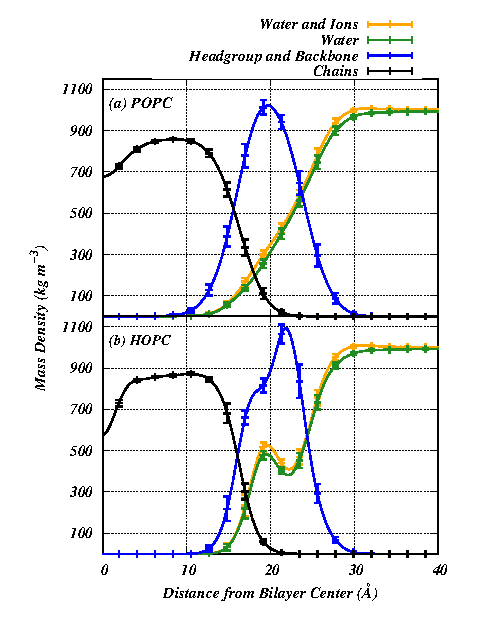
\includegraphics[width=	0.7\textwidth]{dens_3component.eps}
\end{figure}
We find that the headgroup region of 
HOPC has a higher density of solvent compared to POPC -- this is visible as 
a distinct peak in the solvent density profile in the HOPC system. 
We verified that this additional peak does not
result from accumulation of ions by comparing mass density profiles of only water molecules. This
peak is similar to observations of a smaller peak 
made in our previous simulations in the absence of salt,
and may be a direct result of the ether-linked lipids~\cite{kruczek:2017:ether}.

Table~\ref{tab:struc} compares the structural properties of HOPC and POPC bilayers. 
Lipid volumes $V_l = V_c + V_{hg}$, where $V_c$ and $V_{hg}$ are 
\begin{table}
    \caption[Comparison of HOPC and POPC bilayer structure properties.]{ 
Comparison of HOPC and POPC bilayer structure properties: $V_l$ is the lipid
volume; $V_c$ and $V_h$ are the partial volumes of lipids chains and headgroups,
respectively; $2D_c$ and $D_b$ are chain and bilayer thickness, respectively; $A_l=V_c/D_c$ is the area per lipid.
$N_{w}$ is the number of perturbed waters in the system, defined as those behind the \emph{hydration boundary}. $\Delta \nu$ is the quadrupolar splitting constant of each system.}
\label{tab:struc}
\begin{tabularx}{\textwidth}{X|X|X}%{ c|c|c|c }
& POPC with NaCl & HOPC with NaCl \\ \hline
$V_c$ (\AA$^3$) & 898.4 $\pm$ 1.2 & 900.0 $\pm$ 1.0   \\
$V_h$ (\AA$^3$) & 318.9 $\pm$ 0.9 & 290.2 $\pm$ 0.9   \\
$V_l$ (\AA$^3$) & 1217.3 $\pm$ 0.5 & 1190.2 $\pm$ 0.9   \\
$2D_c$ (\AA) & 30.95 $\pm$ 0.32 & 32.13 $\pm$ 0.25   \\
$D_b$ (\AA) & 46.22 $\pm$ 0.49 & 46.05 $\pm$ 0.34   \\
$A_l$ (\AA$^2$) & 58.07 $\pm$ 0.63 & 56.03 $\pm$ 0.45   \\
$D_{hh}$ (\AA) & 40.24 $\pm$ 0.75 & 42.62 $\pm$ 0.88   \\
$N_{w}$ & 22.6 & 22.3  \\ 
$\Delta \nu$ (Hz) & 194.99 & 1756.08 \\
\end{tabularx}
\end{table}
the volumes of lipid chains (tails) and headgroups. 
These are computed using the approach given in 
Petrache et al.~\cite{petrache:1997}. In this approach, 
we first compute the number densities $n_i(z)$ of the various system 
components as a function of the bilayer normal ($z$). We then use these 
$n_i(z)$ to determine their partial molecular volumes, $v_i$, by optimizing the objective function, 
\begin{equation}
\label{eq:petrache}
\Omega(v_i)=\sum^{n_s}_{z_j}(1-\sum_{i=1}^{N_{\text{groups}}}(n_i(z_j)v_i))^2.
\end{equation}
Here, $N_{\text{groups}}=7$ are the different system 
components including methyls ($v_{CH_3}$), methines ($v_{CH_2}$), 
methylenes ($v_{CH}$), headgroup carbons, headgroup and backbone oxygens, headgroup phosphate
and nitrogen, and water ($v_{H_2O}$). 
%These partial volumes are shown in supplemental figure~\ref{supp:tab:volumes}.
Using these partial molecular volumes, we compute 
$V_c = 2v_{CH_3} + 2v_{CH_1} + 28v_{CH_2}$ and $V_{hg} = 10v_{hg_C} + 2v_{P\text{\&}N} + 8v_{hg_O}$. 
We find that the headgroup volume of HOPC is 
27.1~\AA$^3$~smaller than POPC, due likely to the absence of carbonyl groups. 
As expected for lipids with the same
hydrocarbon chains, the chain volumes are similar in the two lipids.

We also use the number densities computed above ($n_i(z)$) to determine lipid chain 
thickness ($2D_c$) and bilayer thickness ($D_b$). These results are found experimentally from 
x-ray and neutron scattering~\cite{fogarty:2015}. In our simulations these parameters 
are found by first computing the probability of
finding the $i$-th group in each slice of the simulation box,
$P_i(z)={n_i(z)}/{\sum_i n_i(z)}$. We define $2D_c$ as the distance between the Gibbs' surfaces on the 
interfacial probability densities of lipid chains. Each of the two surfaces is computed by identifying the
point on the curve where 
the integrals of probability densities in the interfacial regions above and below the surface are equal. 
We compute $D_b$ in a similarly, but from solvent probability densities. 
We find that both POPC and HOPC have similar membrane thicknesses ($D_b$); however a comparison of $2D_c$ 
indicates that the hydrophobic chains in HOPC are slightly thicker than those in POPC, reflecting tighter chain packing. This 
is also evident from comparison of electron densities (see figure~\ref{fig:eledens}). 

\begin{figure}[p]
    \caption[Electron Densities of Simulated Systems.]{ 
Electron Densities of Simulated Systems. Symmetrized electron density distribution of each simulated system as a 
function of $z$. We can see the distribution for HOPC 
is broader, with a longer peak-to-peak distance than in the POPC distribution. Furthermore, 
we see a deeper trough in the middle of the HOPC distribution. This plot was made by using the gromacs densities tool, 
dividing the system into 2000 slices. This data was calculated for every five 
nanoseconds, and averaged over the last 150ns of trajectories. Errorbars are shown for every 10th data point.
}
\label{fig:eledens}
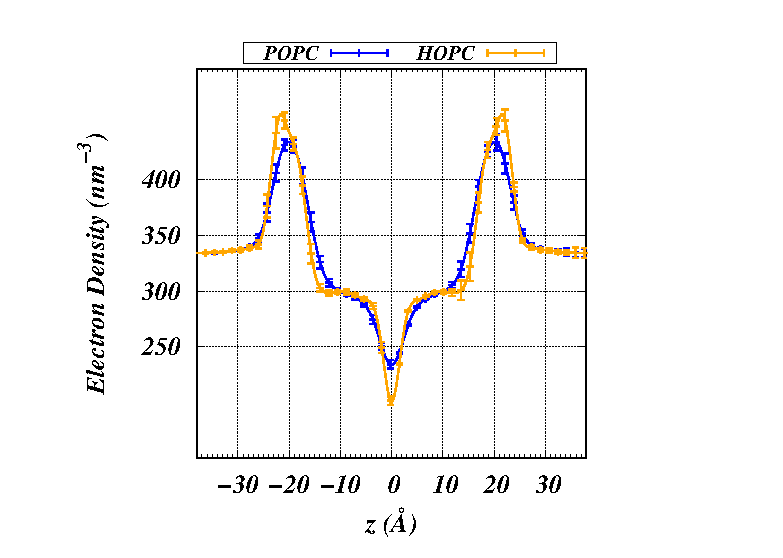
\includegraphics[width=	0.7\textwidth]{ele_scattering_density.eps}
\end{figure}
Electron density distributions are experimentally measured using x-ray scattering, by taking the reverse-fourier transform of
the scattering form-factor~\cite{fogarty:2015,nagle:2000,pandit:2008:simulationtextbook}. Since the experimental x-ray scattering is dependent on the model used to
compute the reverse-transform, we often calculate the form-factor of our simulated bilayer to compare to experiment by transforming the
electron density distribution~\cite{chiu:2009,kruczek:2017:ether,kruczek:2017}.
Since such data is not available for our current lipid system as far as we know, we cannot do this comparison here. 
%We have included this data in supplementary materials in case
%a comparsion becomes possible in the future (see supplemental figure~\ref{supp:formfactor}).

We also use the electron denisty distribution to calculate the peak-to-peak distance $D_{hh}$, 
which is used another measure of the bilayer thickness. This is roughly reflective of the distance between the 
electron-dense phosphate groups on either bilayer leaflet.

$D_{hh}$ values for POPC and HOPC indicate that the ether-linked bilayer is \about2\AA thicker on average than the ester-linked bilayer. 
This discrepancy between the values of $D_b$ and $D_{hh}$ is likely due to the irregular shape of the 
distribution of solvent in the headgroup of HOPC --- the extra region 
of solvent accumulation may move the Gibbs' surface used for finding $D_b$ into the bilayer surface.

The difference in bilayer thickness can also be shown directly from comparison of chain order 
parameters (See figure~\ref{fig:chainorder}). As lipid chains become more ordered on average, bilayer thickness
increases~\cite{nagle:2000}.

\begin{figure}[p]
    \caption[Order parameters of lipid chains.]{ 
Order parameters of lipid chains. Sn$_2$~and Sn$_2$~refer to the two lipid tails. 
The carbon numbering starts from the polar carbon
at the ester bond; however, we do not calculate an $S_{CD}$ for the first carbon as this carbon would not have 
a hydrogen attached in an ester-linked lipid. 
This convention was maintained for the ether-linked lipid. The 
unsaturated bond is between carbons 9 and 10 on the $\text{Sn}_2$ chain.
In both chains, HOPC shows higher ordering, except for the unsaturated carbons on  the 
9-octadecene chain. This ordering corresponds with the lower area per lipid 
of the HOPC bilayer, values of which can be seen in table~\ref{tab:struc}. }
\label{fig:chainorder}
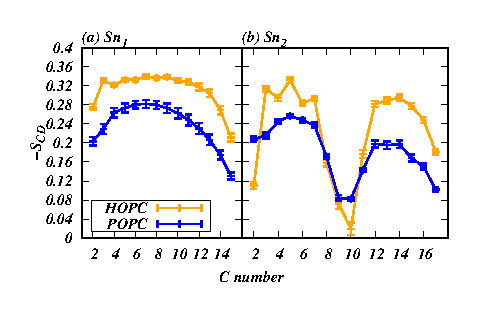
\includegraphics[width=\textwidth]{chainorder.eps}
\end{figure}
We determine chain order parameters from the chain order tensor $S_{\alpha\beta}$ defined as
\begin{equation}
\label{eq:chainorder}
S_{\alpha\beta}=\frac{1}{2}\bigg \langle 3 \cdot \cos(\theta_\alpha) \cdot \cos(\theta_\beta) - \delta_{\alpha\beta}\bigg \rangle\text{,}
\end{equation}
where $\theta_\alpha$ and $\theta_\beta$ are the angles made 
by the molecular axes with $\alpha$ and $\beta$ as either $x$, $y$, or $z$, and $\delta_{\alpha\beta}$ is 
the Kroneker-delta function. For the saturated bonds~\cite{egberts:1988}
\begin{equation}
\label{eq:chainorderparam}
-S^{Sat}_{CD}=\frac{2}{3}S_{xx}+\frac{1}{3}S_{yy},
\end{equation}
and for unsaturated bonds~\cite{douliez:1995}
\begin{equation}
-S^{Unsat}_{CD}=\frac{1}{4}S_{zz}+\frac{3}{4}S_{yy}\mp \frac{\sqrt{3}}{2}S_{yz}
\label{eq:chainordunsat}
\end{equation}
We then use $V_c$ and $D_c$ to calculate areas per lipid, $A_l = V_c / D_c$. We find that the 
lateral surface area of HOPC is slightly smaller than that of the POPC bilayer.

\subsection{Membrane-salt interactions}

Ions prefer to associate or coordinate with specific sites 
in the headgroup regions of the lipid bilayers (See figure~\ref{fig:numberdens}) --- \na ions near 
\begin{figure}[p]
    \caption[Comparison of headgroup component and ion number densities between the HOPC and POPC systems.]{ 
Comparison of headgroup component and ion number densities between the HOPC and POPC systems. The 
inset zooms in on the ordinate axis to visualize the extent of ion 
adsorption into bilayer as well as ion densities in the bulk. Densities are computed by dividing 
the box dimension along the membrane normal into 2000 slices. Error bars are indicated for every 10th slice. 
We note that sodium ions have a broader distribution in POPC than in HOPC. The peak of the \na distribution in 
POPC is also closer to the center of the bilayer than in HOPC. This may be due 
to the interaction of ions with the carbonyl oxygens (shown in red) 
that are present in POPC but absent in HOPC. In both bilayers, the chloride ions 
gather near the positively charged choline trimethylammonium, shown in blue. The 
inset shows the distribution of ions in the transitional region from the bilayer surface to bulk solvent. As one 
looks further out from the bilayer, the density of \na and \cl equalize, as is expected in bulk solvent. 
}
\label{fig:numberdens}
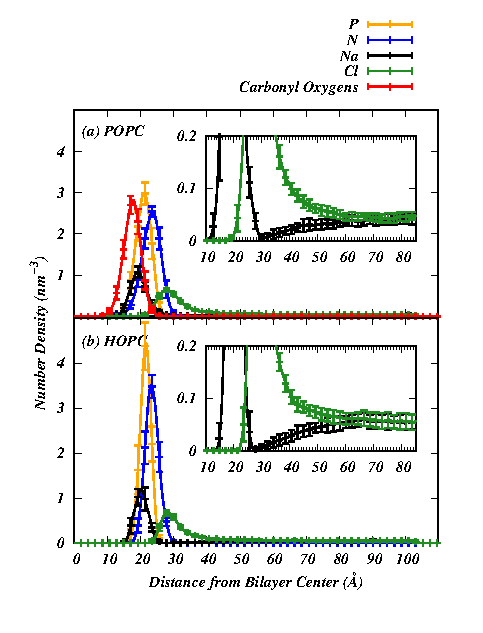
\includegraphics[width=	0.5\textwidth]{density.eps}
\end{figure}
phosphates and \cl ions near cholines. Here we note that ion peaks are positioned similarly in both HOPC and 
POPC systems. \cl ions do not enter the bilayer headgroup region, while \na ions move far into this region
of the bilayer surface. However, the \na densities trail off deeper into the POPC bilayer by 
$\sim5$~\AA~(visible in the inset of figure~\ref{fig:numberdens}). 
In fact, we find that more ions localize in the POPC bilayer --- Averaged over the last 150 ns we see
$74.45 \pm 0.56$ \na  
ions bound to POPC, 
compared to 
$62.27\pm 2.00$ \na ions bound to HOPC.
We consider an ion to be bound to the membrane when half or fewer of the inner-shell coordination partners of the 
ion are waters. The inner shell of \na ions is defined using a cutoff of 3.15~\AA~based on radial distribution functions of \na with the water oxygens~\cite{varma:2008:JACS}.
The \cl ions do not lose waters and do not seem to adsorb on the bilayer, hence we have not analyzed
the binding behavior of \cl in this work.
Figure~\ref{fig:cationcood} shows the inner-shell coordination environment of \na ions as a 
function of their positions in the bilayer. 
\begin{figure}[p]
    \caption[First shell coordination environment of \na ions.]{ 
First shell coordination environment of \na ions. The cutoff distance for the first shell is taken as 3.3 
\aangstroms, based on the radial distribution function of \na with the various lipid oxygens.
This chart was made by dividing the box into 400 slices, and then symmetrizing around the bilayer 
center. Data is averaged over the last 100ns of simulation trajectory. Errorbars are shown for every tenth data point. 
Note that the coordination number of \na drops from 6 to 5 as it interacts deeper in both bilayers, and
this drop occurs sooner in the HOPC system than in POPC. 
No values are shown for at distances less than $7.5$~\AA~from the bilayer center, due to the lack of ions beyond in this region. 
}
\label{fig:cationcood}
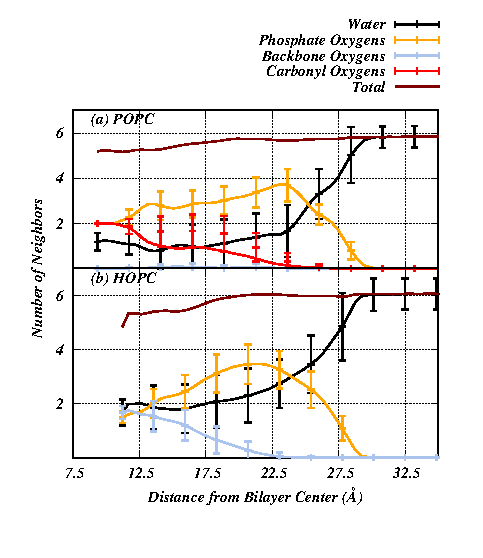
\includegraphics[height=0.66\textheight]{cood.eps}
\end{figure}
For this, we used a cutoff
of 3.3~\AA, based on the radial distrubution functions of \na with the
various lipid oxygens (data not shown). When \na ions are bound, they are primarily coordinated by 
phosphate oxygens --- this holds for both HOPC and POPC. The main difference between POPC and HOPC is 
in how carbonyl oxygens, backbone oxygens, and water oxygens coordinate with ions. In POPC, ions are partially 
coordinated by both carbonyl oxygens and water, but not by backbone oxygens; however, in HOPC backbone oxygens do partially coordinate \na. 
This may contribute to the deeper penetration of \na into the POPC bilayer, and the greater number of ions adsorbed onto the POPC
bilayer surface when compared to HOPC.

\subsection{Water structure and dynamics}
\label{sec:waterstruc}
As we noted above in Figure~\ref{fig:massdens}, the headgroup region of HOPC has a higher density of water than 
POPC. We have also noted previously that in 
general salts tend to extend the region of structured water near the bilayer surface~\cite{kruczek:2017}. 
To gain further insight into how the absence of carbonyl groups in ether lipid bilayers increases water density, we systematically characterize the structure and dynamics of water.  

Figure~\ref{fig:hrdf} compares the integrated radial distribution of water hydrogens around lipid oxygens. 
\begin{figure}[p]
\caption[Cumulative radial distribution functions of water hydrogens around
various lipid oxygens.]{ 
Cumulative radial distribution functions of water hydrogens around
various lipid oxygens. The distributions for POPC are shown in solid lines, while HOPC is shown with dotted lines. 
The oxygens are grouped into categories as denoted in figure~\ref{fig:struc}.}
\label{fig:hrdf}
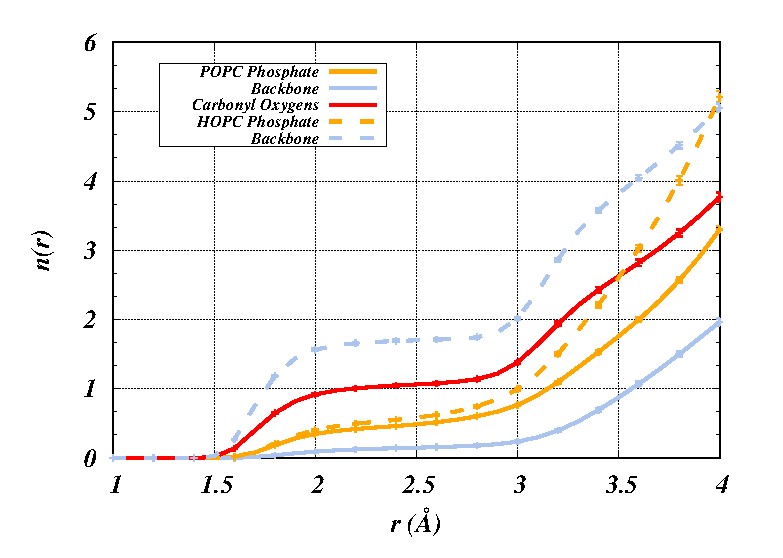
\includegraphics[width=\textwidth]{h_rdf_cum.eps}
\end{figure}
We note that there is very little water directly coordinating the backbone oxygens in the POPC bilayer (\about $1/3$ water per lipid). 
Compared to backbone oxygens, more water directly coordinates the ester carbonyl oxygens and the phosphate oxygens in POPC. 
We see a larger number of waters coordinating with the backbone oxygens in HOPC than in POPC, nearly $2$ waters per lipid.
Therefore, we attribute the higher density of water in HOPC to coordination with backbone oxygens. 

Note that in POPC, carbonyls oxygens compete with phosphates for water coordination. Consequently, we expect waters 
to have a greater average ordering in the HOPC headgroup. We had observed this greater ordering in our previous comparative study of 
diether- and diester-lipid bilayers \cite{kruczek:2017:ether}. 


In order to further explore solvent ordering by the bilayer surface, we compute order parameters of water O-H bonds.
The first order parameter ($P_1$) is calculated by time-averaging the cosine of 
the angle $\theta$ that the OH bond makes with the bilayer normal, 
that is $P_1 = \langle \cos(\theta) \rangle$. Consequently, a positive value represents an orientation 
away the bilayer. The second parameter, which is defined as the second Legendre polynomial of $\cos(\theta)$, that 
is, $P_2 = \langle (3 \cdot \cos^{2}(\theta)-1) \rangle/2$.  
We calculate both $P_1$ and $P_2$ as a function of position along the bilayer normal, and they are shown in figure~\ref{fig:h2order}. 

\begin{figure}[p]
    \caption[The first and second order parameters, $P_1$ and $P_2$, of water O-H bonds.]{ 
The first and second order parameters, $P_1$ and $P_2$, of water O-H bonds. Each parameter is calculated by first dividing the simulation box into 2000 slices, 
and then averaging the data separately in each slice. The box is symmetrized around the bilayer center, and thus 
only half the box is shown. Standard deviations are calculated by dividing 
the trajectory into over 5ns blocks. The dashed vertical lines in the $P_2$ 
plot are demarkations for the different spatial regions, $B_{-1}$, $B_{+}$, $B_{-2}$, and $B_\text{bulk}$, as discussed in the associated text.
$P_1$ is the average of the first legendre polynomial of the cosine of the angle between the bilayer normal and the O-H bond vector of each water molecule per box slice. 
$P_2$ is the average of the second legendre polynomial.
Looking to $P_1$, both systems exhibit similar magnitudes of ordering. $P_2$ shows a more complicated distribution, with larger magnitudes of ordering in all regions in the HOPC system.}
\label{fig:h2order}
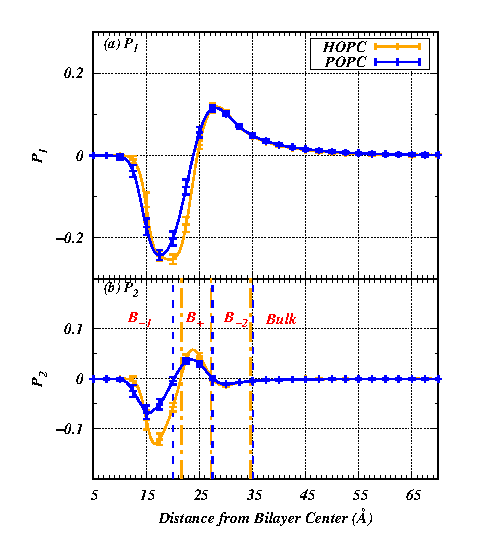
\includegraphics[height=0.66\textheight]{h2order.eps}
\end{figure}
We find that the water in the headgroup region is clearly more ordered in the HOPC bilayer.  
Figure~\ref{fig:h2order}b shows the second order parameter. We note that the induced perturbations in the water layer are more prominent in HOPC than that of POPC.
At the same time, however, we find that the numbers of water that are ordered in the two systems are similar.
We count the average number of non-bulk (perturbed) waters as waters within the non-zero region of the second order parameter. 
We find this boundary by fitting an exponential function to the region starting at the peak in
the first order parameter, and taking the inverse of the length-scale of the fitted function as the position of the surface.
The region beyond this point is considered bulk water. We will refer to this surface as the \emph{hydration boundary} for the remainder of the paper.
For the purpose of counting the number of waters in the surface, we truncated the box at this boundary, to a length of 35 \aangstroms. 
Numbers of perturbed waters per lipid for each system can be seen in table~\ref{tab:struc} line 8.

We also use these order parameters to compute the quadrupolar splitting of water as measured in NMR experiments. 
It is essentially a weighted average of the second order parameter, similar to the one derived by Kruczek \etal~\cite{kruczek:2017:ether}: %\AA man\etal~\cite{aaman:2003}:
\begin{equation}
\label{eq:deltanu}
\Delta \nu = \frac{3}{4} \chi \frac{1}{N_{\text{w}}}\sum^{z_0}_{z_i=0}n_{w}(z_i)P_2(z_i),
\end{equation}
where the number of perturbed waters in the system is $N_\text{w}$, $n_{w}$ is the number of waters in each slice of the box,
and $P_2(z_i)$ is the value of the second order paramter in the $i^{\text{th}}$~slice. We take the quadrupolar splitting constant of water $\chi=220 \text{KHz}$ 
from~{\AA}man \etal~\cite{aaman:2003}. 
The summation over slices is carried out from the bilayer center ($z=0$) to 
the end of the box. 
We report that the quadrupolar splitting of water in the POPC system is 194.99 Hz, and that in the HOPC system is 1756.08 Hz (also shown in table~\ref{tab:struc}, line 9). 
These values reflect a similar difference to what we observed in our earlier comparative study of ether- and ester-linked lipid bilayers in pure water~\cite{kruczek:2017:ether}.

Next we compute the lateral diffusion coefficient of water. To gain detailed insight, we compute it 
separately for four different regions along the bilayer normal. We define these regions 
using the $P_2(z)$ profile: $B_{-1}$ is the region closest to the bilayer center where 
$P_2(z)$ is negative; $B_{+}$ is the region where $P_2(z)$ 
is positive; $B_{-2}$ is the region beyond the $B_{+}$ boundary where $P_2(z)$ is 
negative; and the remaining portion beyond $B_{-2}$ we refer to as bulk. 
These regions are also labeled in figure~\ref{fig:h2order}. The diffusion coefficients for waters 
in these regions are included in table~\ref{tab:diff}. They are calculated using Einstein's relationship, and a 
\begin{table}[t]
\caption[Diffusion coefficients of water measured in $\text{nm}^2/\text{s}$ in different regions along the bilayer normal (see figure~\ref{fig:h2order} 
and related text for the definitions of the different spatial regions.]{
Diffusion coefficients of water measured in $\text{nm}^2/\text{s}$ in different regions along the bilayer normal (see figure~\ref{fig:h2order} 
and related text for the definitions of the different spatial regions.
The two innermost-bilayer regions $B_{-1}$ and $B_+$ in HOPC contain waters that have a greatly lowered diffusion coefficient. In the regions $B_{-2}$ and bulk, 
the bilayer composition does not seem to change the diffusion behavior. These values were calculated using the method outlined in previous work by our lab~\cite{kruczek:2017:ether}
The various regions are illustrated on figure~\ref{fig:h2order}.
}
\label{tab:diff}
\begin{tabularx}{\textwidth}{X|X|X|X|X|}%{c|c|c|c|c}
& $B_{-1}$ $(nm^2/s)$ & $B_+$ $(nm^2/s)$ & $B_{-2}$ $(nm^2/s)$ & Bulk $(nm^2/s)$\\ \hline
HOPC & 0.85 \PM 0.59 & 1.783 \PM 0.94 & 16.1 \PM 5.24 & 26.67 \PM 0.65 \\
POPC & 1.075 \PM 0.62 & 3.078 \PM 0.74 & 16.27 \PM 5.19 & 27.30 \PM 0.66 \\
\end{tabularx}
\end{table}
protocol detailed in our previous study~\cite{kruczek:2017:ether}. Taking note of the overall pattern, the 
lateral diffusion decreases progressively as one moves deeper into the bilayer. Additionally, in the innermost 
regions $B_{-1}$ and  $B_+$ water diffuses more slowly in HOPC compared to POPC. This result 
is similar to what we observed previously~\cite{kruczek:2017:ether} in simulations without salt.

To characterize the orientational dynamics of waters, we compute autocorrelations of the O-H bonds,
\begin{equation}
\label{eq:autocorr}
C^{O-H} (t) =\bigg \langle \vec{v}_{O-H}(0) \cdot \vec{v}_{O-H}(t) \bigg \rangle\text{.}
\end{equation}
We calculate expectation values separately for all the 2~\AA~slices along 
the bilayer normal by tracking individual water molecules for 500ps, and also averaging over all 
waters in the slice. We also weight each water by the fraction of duration it spends in each slice. This is done in 5~ns chunks, and then averaged over the trajectories. 
We then model these autocorrelations as a sum of three exponential terms,
\begin{equation}
\label{eq:fit}
C^{O-H} (t) = A_1 e^{-t/\tau_1} + A_2 e^{-t/\tau_2} + (1 - A_1 - A_2) e^{-t/\tau_3}\text{,}
\end{equation}
where $A_i$ are positive, and $\tau_i$ are correlation times. Fitting is carried out using the 
Marquardt-Levenberg least-squares fitting method. The correlation times are plotted in figure~\ref{fig:waterautotime}. 

\begin{figure}[p]
    \caption[Orientational autocorrelation times of O-H bonds in water, as determined by modeling their autocorrelations using three-exponential fits.]{ 
Orientational autocorrelation times of O-H bonds in water, as determined by modeling their autocorrelations using three-exponential fits. 
No values are shown for at distances less than $12$ \AA~from the bilayer center, as there are no waters in this region. 
The dashed vertical lines indicate chain boundaries $D_c$ and bilayer thickness $D_b/2$, colored to indicate the lipid system.}
\label{fig:waterautotime}
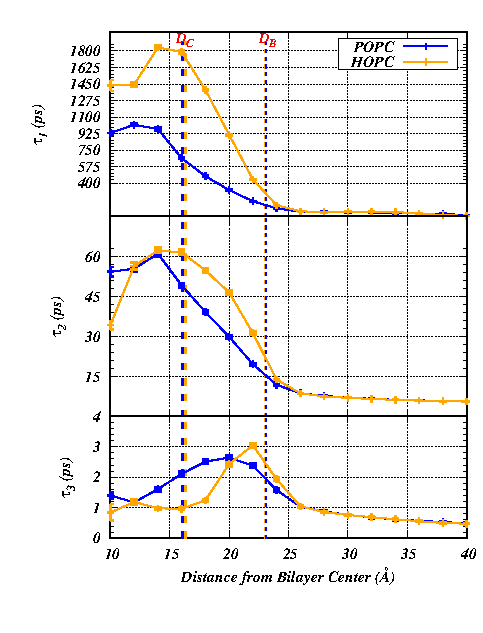
\includegraphics[height=0.66\textheight]{Corrtime}
\end{figure}
We find that $\tau_1$ shows a profile similar to what we observed for ether- and ester-lipids 
simulated in pure water~\cite{kruczek:2017:ether}. Additionally, we find that the correlation times $\tau_1$ and $\tau_2$ in the 
HOPC bilayer are all longer than in POPC. The maximum correlation times of 1838 ps in HOPC and 1019 ps in 
POPC are characteristic of rotationally immobile waters inside the bilayer surface 
and also of crystallographically-resolved waters in 
protein-protein interfaces \cite{dutta:2014}. Note that $\tau_3$, which 
is of the order of picoseconds, is close to the sampling time of our trajectories. Thus, we regard it simply as a fitting parameter.

Overall, we find that the headgroup water in HOPC is significantly more organized and also diffuses more slowly as compared 
to the headgroup water in POPC. This is similar to what we had 
observed~\cite{kruczek:2017:ether} when we compared another diether lipid 
bilayer against its chemically analogous diester-lipid bilayer, but in the absence of NaCl. 
This leads us to conclude that in ether-linked lipid bilayers water forms a rigid and immobile layer within the headgroup region of the bilayer,
and exposure to a moderate concentration of salt does not disrupt this layer.%; this keeps the bilayer more rigid than the ester-linked analogue.

\subsection{Bilayer electrostatics}

The dipole potential of a bilayer is the potential difference between the inside of the bilayer 
and bulk water. In our previous comparative study of ether- and ester-linked bilayers in pure water\cite{kruczek:2017:ether} 
we had found that the dipole potential of the ether-linked lipid bilayer was $56 \pm 5$ mV smaller 
than that of the ester-linked lipid bilayer, and this finding was consistent with experiment~\cite{gawrisch:1992}. 
We also know that membrane association with salt can modify its dipole potential, with increases
of around 200mV from that of a bilayer without salt reported previously~\cite{kruczek:2017,Berkowitz:2006,Cordomi:2008}.

Figure~\ref{fig:epot} compares the electrostatic potential in HOPC and POPC 
as a function of distance along the bilayer normal. 
\begin{figure}[p]
    \caption[Comparison of electrostatic potentials between the HOPC and POPC systems.]{ 
Comparison of electrostatic potentials between the HOPC and POPC systems. 
These distributions are calculated by integrating the charge density of our systems twice, assuming the potential goes 
to zero at the box edge and that the electric field of bulk solvent is zero. 
Looking to the region from the bilayer center to around 10~\AA, one can see 
the bilayer dipole potential. We see very similar values for this in 
both systems. We also see a large peak in the HOPC system, 
and a large trough that is not present in POPC. The larger peak at the bilayer surface may provide a barrier to  
solvent and dissolved ions, and the trough may be a trap that causes the buildup of solvent in the bilayer headgroup region. }
\label{fig:epot}
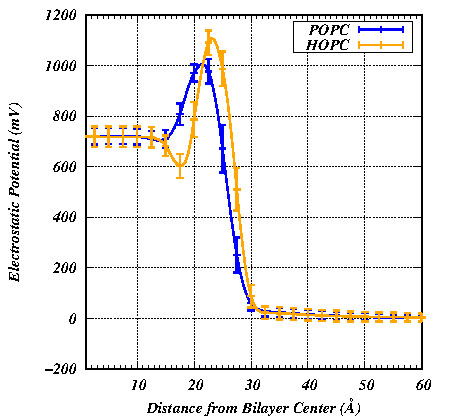
\includegraphics[width=\textwidth]{potential}
\end{figure}
These are calculated from an integration of the one dimensional Poisson's equation,
\begin{equation}
\label{eq:poissonint}
\phi(z)=-\frac{1}{\epsilon_0}\int_{0}^{z}\int_{0}^{z'}\rho(z) dz dz' + C_1z + C_2,
\end{equation}
where $\rho(z)$ is the charge density along the bilayer normal, and $\epsilon_0$ is the 
vacuum permittivity. Note that we integrate this equation using two boundary 
conditions --- the electric field in bulk water is zero, yielding $C_2=0$, and 
the potential at the simulation box boundary is also zero, which makes $C_1=0$.

The first observation we make is that the 
dipole potentials of both HOPC and POPC are similar; a behavior distinct from that 
observed in simulations in pure water. Nevertheless, the overall electrostatic potential 
profiles are similar to those observed in pure water. Firstly, a characteristic peak near the 
phosphate region still exists, and this peak is higher for the diether lipid bilayer. This could potentially 
serve as a higher permeation barrier in the diether-linked lipid system. This interpretation is consistent with our 
observation above that there are fewer membrane-associated ions in HOPC compared to POPC. Secondly, the 
diether-linked lipid system had a trough next to the peak, which is absent in the diester-linked lipid bilayer, and 
may serve as a trap for solvent molecules. In fact, the spatial location of the trough corresponds to the high water density region in the HOPC bilayer.


%Another barrier to ions would lie in the ability for the ions to polarize their surroundings within the bilayer.
%The lipid headgroup dipoles are relatively stiff, so ions must depend somewhat on the solvent that is inside
%the bilayer to lower their free-energy. The ease by which the solvent can be polarized is shown in the dielectric
%constant of the material. We calculated this per each 
%slice of the simulation box using the Clasius-Mossoti-like equation shown below:
%\begin{equation}
%\label{eq:diele}
%\epsilon_r(z) = 1 + \frac{\langle M_{slice}^2 \rangle - \langle M_{slice} \rangle ^2}{3\epsilon_0 K_b T \langle V_{slice} 
%\rangle }
%\end{equation}
%Where $M_{slice}$ is the total dipole moment from water molecules in each slice, $\epsilon_0$ is the 
%permittivity of free space, $K_b$ is Boltzmann's constant, $T$ is the target thermostat temperature, 
%and $V_{slice}$ is the volume of each slice. The expectation values were taken over 5ns chunks of time,
%and the distribution was averaged over the last 150ns of simulation. The plot can be seen in figure~\ref{fig:diele}.

%\section{Simplified Model of the Interface; Gouy-Chapman Theory}
\subsection{Salt distribution at the bilayer-solvent interface}

The behavior of salt near bilayer surfaces is often modeled using Gouy-Chapman theory; 
a mean-field approximation that has its roots in Poisson-Boltzman theory~\cite{israelachvili:2011:intermol,wiersema:1966}. 
This theory also forms the basis for electrophoretic mobility studies~\cite{wiersema:1966,o:1978:electrophoretic}. 
In this theory, water is modeled as 
a dielectric continuum in which ion particles behave as an uncorrelated gas. This means that the number density distribution of ions in the dielectric continuum only
depends on the temperature and the electrostatic potential applied to the system.

So far, due to limitations from system size and ionic force field parameters, 
we have refrained from comparing or validating our simulations at the atomistic level against this theory. 
Here, we show convergence between these atomistic simulations and the Poisson-Boltzman theory.  

Within Poisson-Boltzmann theory, the number density of ions near the bilayer surface is described as
\begin{equation}
\label{eq:gcnum}
\rho(z) = \rho_0 \exp\big({- \bar z \text{\si{\elementarycharge}} \beta \psi(z)}\big),
\end{equation}
where $\rho_0$ is the ion density in the bulk, $\bar z$ is the valency of the ion, $\beta = (k_bT)^{-1}$, \si{\elementarycharge} is the charge 
on an electron, and $\psi(z)$ is the electrostatic potential. We define the interfaces as the 
\emph{hydration boundaries} (see subsection~\ref{sec:waterstruc} `Water structure and dynamics'). The lengths of the solvent 
occupied regions, $D$, in each of the two systems are listed in table~\ref{tab:gctheory}. We set the center 
\begin{table}
    \caption[Parameters in Gouy-Chapman theory.]{ 
Parameters in Gouy-Chapman theory. 
$K$ was calculated using equation~\ref{eq:debyelength}. This was done using the value for $\rho_0$  
for each system, found by taking the average number density of \cl ions within 
the solvent-occupied region of the box. The charge density $\sigma$  was 
calculated by integrating the charge of the ions from the bilayer center to the surface at 35 Å 
from the bilayer center for each system, shown to be the \emph{hydration boundary} of both bilayers. $D$ gives the length of the solvent-occupied region of each simulation box.
}
\label{tab:gctheory}
\begin{tabularx}{\textwidth}{X|X|X|X|X|}
    & $K$(\invnm) & $D$ \nmeter & $\rho_0$ (\si{\nm\tothe{-3}})& $\sigma$ (\si{\elementarycharge\nm\tothe{-2}}) \\\hline
POPC&$0.98$\added{$\pm0.021$}&$13.167$\added{$\pm0.0071$}&$0.043$\added{$\pm0.0018$}&$0.13$\\
HOPC&$1.09$\added{$\pm0.037$}&$13.752$\added{$\pm0.0068$}&$0.060$\added{$\pm0.0041$}&$0.128$   \\
\end{tabularx}
\end{table}
of this solvent occupied region as $z=0$, which then implies that the interfaces are essentially 
at $z=\pm D/2$~nm, as illustrated in figure~\ref{fig:gctheoryimg}. 
\begin{figure}[p]
    \caption[Illustration of bulk ion distribution, with surfaces used in Gouy-Chapman theory
calculations.]{ 
Illustration of bulk ion distribution, with surfaces used in Gouy-Chapman theory
calculations. For the purpose of illustration, solvent has been hidden from this image. \cl ions have been
colored in green, and \na ions are shown in red. Surfaces set at the \emph{hydration boundary} of each
bilayer leaflet are shown with dotted lines. The center of the solvent occupied region of the box is set at zero.}
\label{fig:gctheoryimg}
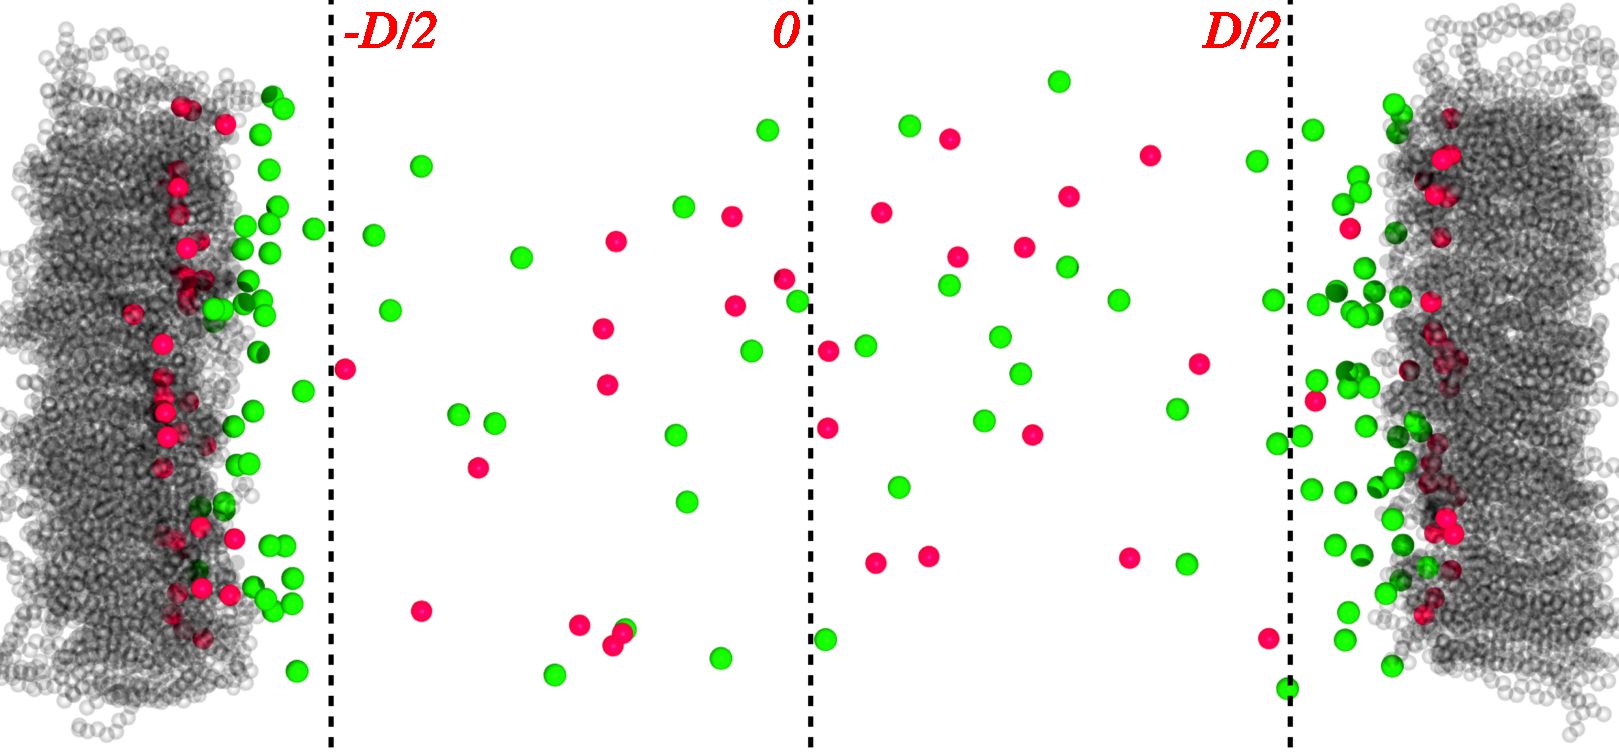
\includegraphics[width=\textwidth]{images/GCTheory_image.eps}
\end{figure}
We model $\psi(z)$ as a sum of two Debye-Huckle 
potentials~\cite{israelachvili:2011:intermol}, each a reflection of the other around the center of the solvent occupied region:
\begin{align}
&\psi_{1}(z) = \psi_s \exp\bigg({-K(z+\frac{D}{2})}\bigg)\\
&\psi_{2}(z) = \psi_s \exp\bigg({K(z-\frac{D}{2})}\bigg)\\
\label{eq:gcpot}
&\psi(z) = \psi_1(z) + \psi_2(z) - \big({\psi_1(0)+\psi_2(0)}\big)
\end{align}
Here $\psi_s = \sigma/\epsilon_0\epsilon K$ is the electrostatic potential at the bilayer surface, where $\sigma$ 
is the surface charge density of the bilayer leaflet~\cite{israelachvili:2011:intermol}. $K$ is the inverse Debye length, 
\begin{equation}
\label{eq:debyelength}
K=\sqrt{\sum_{i} \rho_{0,i} \bar z_i^2\frac{\text{\si{\elementarycharge}}^2}{\epsilon_0 \epsilon k_bT}},
\end{equation}
where the sum of $\rho_{0,i}$'s is over all the included ions in our system. Note that in Equ.~\ref{eq:gcpot} we 
subtract out the value of the potential at the center of the solvent occupied region from $\psi(z)$. 
Note also that the form of $\psi_s$ is valid only for small surface potentials, generally those smaller than 
20 millivolts~\cite{israelachvili:2011:intermol}. Our systems have a relatively small surface charges 
(See table~\ref{tab:gctheory}), 
which will result in small surface potentials (See table~\ref{tab:gctheory}). 
The surface charges are calculated by integrating 
charge densitities of ions contained behind the surface. We chose to do this because all other parts of 
the simulated system are uncharged, and the surface is entirely charged by the adsorbed ions.

Figure~\ref{fig:gctheory} compares the potential and ion distribution 
obtained from theory against those estimated directly from simulations. 

\begin{figure}[p]
    \caption[Comparison of Gouy-Chapman theory predictions and simulation results.]{ 
Comparison of Gouy-Chapman theory predictions and simulation results. Theoretical distributions are given by the 
solid lines, and data from our simulations are shown as points with error bars. (a) and (c) show the electrostatic
potentials of each system. For clairity, we show error-bars for the simulation
results for every 13th point. The Debye-Huckle 
potentials shown follow the form given in equation~\ref{eq:gcpot}. (b) and (d) show the number density distribution
of ions in each system. Error-bars for the 
simulation results are shown
for every 30th point. Note that both systems are
translated to center around the solvent-occupied region of the box, giving an interspace region of \about 13 nm in
each system. Parameters used in Gouy-Chapman theory are in table~\ref{tab:gctheory} }
\label{fig:gctheory}
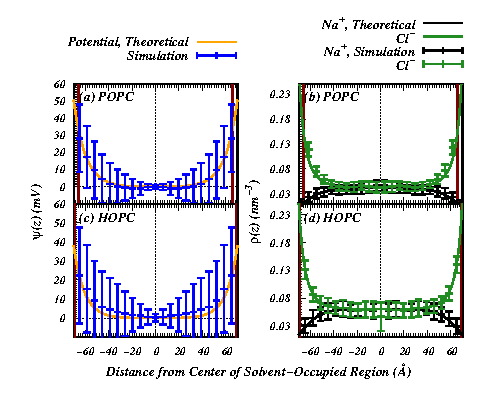
\includegraphics[width=\textwidth]{gouy.eps}
\end{figure}
We note a very close match between the two. Additionally, we find that HOPC shows a slightly 
larger $K$ than POPC, indicating a \about10\% 
shorter screening length for the system. This means that a bilayer of HOPC is better shielded from environmental electric fields.
The shorter screening length in the HOPC is also reflective of the smaller 
number of ions that adsorb onto the surface of the bilayer, as this directly results in a larger number density in bulk solvent due to the fixed number of ions in our system.

\chapter{Conclusions}
Phospholipids are an important part of all living things, acting as the major constituent of cellular plasma membranes. 
The great variety of phospholipid species allows organisms another parameter
to fine-tune the behavior and structure of their membranes in order to adapt to a wide range of different
environments~\cite{van:2008:lipidvariety}.
Ether-linked lipids are a major distinguishing feature of archael membranes, have been suggested in the past to be an adaptation to archaeal membranes to tune
flexibility and permeability of their membranes to extreme environments~\cite{koga:2014,valentine:2007}.

In our work, we have found that ether-linked lipid bilayers show a distinct peak in solvent density
that is not disrupted by the inclusion of a moderate concentration of salt. This region
shows siginificantly reduced lateral diffusion, and longer autocorrelation times than the same
region in an analgous ester-linked lipid bilayer. Furthermore, we find that
the characteristic lower dipole potential of an ether-linked bilayer reported in previous work~\cite{kruczek:2017:ether} is 
increased to match that of the ester-linked bilayer in the presence of salt. We also find that,
with our new protocol for determining the interface boundary of the lipid bilayer,
our simulations model ion distributions and electrostatic potentials from Gouy-Chapman theory well. 
The shorter screening length in the
ether-linked system suggests better shielding from electric fields far 
from the bilayer compared to the ester-linked system. This is a result
of the ether-linked lipid bilayer's lower affinity for ions than the ester-linked analog.

%Early prokaryotes and archaea distinguished themselves from the other
%kingdoms of life in part by their choice between ether- and ester- linked lipids. It has
%been suggested that the move towards
%ether-linked lipids may have been an adaptation to the stress felt by archaea living in
%extreme environments, allowing them to thrive~\cite{valentine:2007}. In our work, we 
%have sought to characterize the differences between an ether-linked lipid bilayer of HOPC and an
%ester-linked analog, POPC, in the presence of dissolved NaCl salt. These systems were simulated
%using the gromos 43A1-S3 lipid force field
%developed by our group~\cite{chiu:2009}, and the ion parameters
%developed by Joung and Cheatham III~\cite{joung:2008}. Both sets of parameters have been demonstrated
%in our previous works~\cite{kruczek:2017,kruczek:2017:ether}. 

%We have found that the HOPC bilayer is thicker than POPC, with a lower area per lipid and a larger bilayer
%thickness, a result that has been seen in previous work~\cite{kruczek:2017:ether}. 
%We found that ions penetrate more into the headgroup region of the POPC bilayer than in HOPC. We also found
%that in HOPC bilayers we observe the mobility of solvent significantly arrested by interaction with the
%lipids, and is apparently not changed by the introduction of ions to the system. If anything,
%the effect in the systems with ions appears to be much greater than results from systems without for both
%ether and ester linked lipids alike~\cite{kruczek:2017:ether}. 
%
%We used our simulations to predict that HOPC has a large peak in its electrostatic potential near the bilayer surface, larger
%than in POPC. This seems unchanged by the introduction of ions, as this was seen without ions in ether-linked lipid
%bilayers. What does change is that the bilayer dipole potential for both HOPC and POPC are now equal. In both simulation
%and experiments on ether-linked bilayers, it has been reported that the dipole potential of ether-linked lipid
%bilayers is lower than that of ester-linked lipids~\cite{kruczek:2017:ether,gawrisch:1992}. We also see a trough in the electrostatic
%potential of HOPC that is not present in POPC, that may act as a trap for ions in the headgroup region. This may prevent ions from moving
%deeper into the HOPC bilayer. This feature has been seen in systems without salt in the past~\cite{kruczek:2017:ether}.
%Finally, we find that the Debye screening length of the HOPC system is shorter than in POPC, indicating that
%the system may be better shielded against electric fields from away from the bilayer.

%\section{Acknowledgements}
%Computing support was sponsored in part by NSF MRI CHE-1531590, CNS-1513126 and IIS-1253980. \\
%Author SV acknowledges partial support provided NIH under the grant number R01GM118697.
\bibliography{refs}
%\newpage
%\section{Supplemental Figures and Captions}
%\beginsupplemental
%Figure~\ref{supp:scatdensity}: Neutron scattering
%length densities from simulation. 
%This is calculated assuming a 
%50\% deuterium concentration, however we do
%not simulate our systems with deuterated water. 
%We can see a peak in the HOPC distribution
%that corresponds with the water density peak in 
%figure~\ref{fig:massdens}. We also see a deeper trough in
%HOPC, again indicating less interdigitation of the lipid
%chains.
%
%~\\
%\added{
%Table~\ref{supp:tab:volumes}: Component volumes calculated from
%number densities using the method
%outlined by Petrache \etal~\cite{petrache:1997}. Values for each headgroup component are difficult to 
%determine uniquely due to significant overlap in their number density distribution, as well as the volume per each $CH_1$ group.
%}
%
%Figure~\ref{supp:formfactor}: X-ray scattering
%formfactors from simulated systems. These are the cosine
%transform of the electron densities for POPC (a) and HOPC (b).
%~\\
%\clearpage
%\clearpage
%
%\begin{table}
%\caption{ }
%\label{supp:tab:volumes}
%{\footnotesize
%\begin{tabularx}{\textwidth}{X|X|X|X|X|X|X|X|X}
%&Water \& Ions & P\&N & HG Oxygens & HG Carbons & CH$_2$ & CH$_1$ & CH$_3$  \\\hline
%HOPC&29.96 $\pm$ 0.003989 & 24.43 $\pm$ 0.5058 & 2.589 $\pm$ 0.4493 & 22.59 $\pm$ 0.3381 & 26.57 $\pm$ 0.06971 & 23.9 $\pm$ 0.4969 & 53.98 $\pm$ 0.2396 \\
%POPC&29.99 $\pm$ 0.002374 & 20.61 $\pm$ 1.045 & 8.651 $\pm$ 0.2112 & 20.84 $\pm$ 0.3946 & 26.5 $\pm$ 0.1096 & 24.28 $\pm$ 0.685 & 53.72 $\pm$ 0.408 \\
%\end{tabularx}
%}
%\end{table}
%
%\clearpage
%
%\begin{figure}
%\caption{ }
%\label{supp:formfactor}
%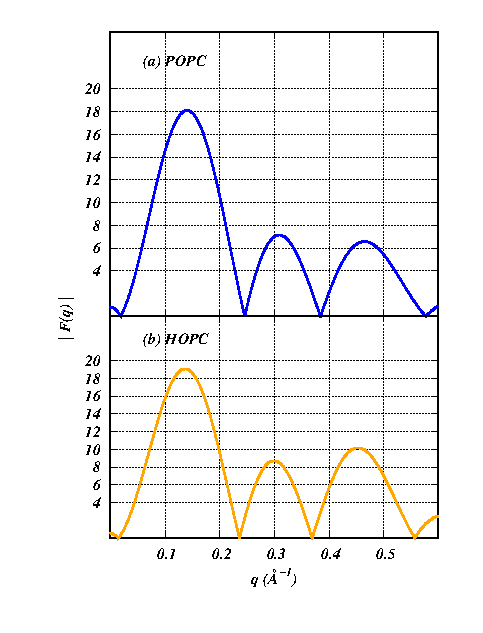
\includegraphics[width=\textwidth]{formfactor.eps}
%\end{figure}
%\clearpage
%\FloatBarrier
\end{document}
